\documentclass[conference]{IEEEtran}
\IEEEoverridecommandlockouts
% The preceding line is only needed to identify funding in the first footnote. If that is unneeded, please comment it out.
%Template version as of 6/27/2024

\usepackage{cite}
\usepackage{amsmath,amssymb,amsfonts}
\usepackage{algorithmic}
\usepackage{graphicx}
\usepackage{textcomp}
\usepackage{xcolor}
\usepackage{hyperref} 
\usepackage{circuitikz}
\usepackage{float}
\usepackage{subcaption}
\graphicspath{{image/}}


\providecommand{\TDMA}{
\begin{circuitikz}
        \tikzstyle{every node}=[font=\fontsize{10.2pt}{13.3pt}\selectfont]
        \draw  (0.5,12.875) rectangle (2.5,11.25);
        \draw  (2.5,12.875) rectangle (4.5,11.25);
        \draw  (4.5,12.875) rectangle (6.5,11.25);
        \draw  (6.5,12.875) rectangle (8.5,11.25);
        \draw  (8.5,12.875) rectangle (10.5,11.25);
        \draw [short] (0.5,13.25) -- (10.5,13.25);
        \draw [short] (0.25,13) arc[start angle=178.78, end angle=91.22, radius=0.2555];
        \draw [short] (10.5,13.25) arc[start angle=90.00, end angle=0.00, radius=0.2500];
        \draw [short] (10.625,13.625) -- (10.625,13.625);
        \draw [short] (10.625,13.625) -- (10.625,13.625);
        \draw [short] (5.75,14) -- (5.75,14);
        \draw [short] (5.75,14) -- (5.75,14);
        \draw [short] (5.875,13.875) -- (5.875,13.875);
        \node [font=\fontsize{18.2pt}{23.7pt}\selectfont, inner xsep=0.080cm, inner ysep=0.085cm, rounded corners=0.020cm] at (5.5,13.625) {Frame};
        \node [font=\fontsize{18.2pt}{23.7pt}\selectfont, inner xsep=0.080cm, inner ysep=0.085cm, rounded corners=0.020cm] at (1.5,12) {T1};
        \node [font=\fontsize{18.2pt}{23.7pt}\selectfont, inner xsep=0.080cm, inner ysep=0.085cm, rounded corners=0.020cm] at (3.5,12) {T2};
        \node [font=\fontsize{18.2pt}{23.7pt}\selectfont, inner xsep=0.080cm, inner ysep=0.085cm, rounded corners=0.020cm] at (5.5,12) {T3};
        \node [font=\fontsize{18.2pt}{23.7pt}\selectfont, inner xsep=0.080cm, inner ysep=0.085cm, rounded corners=0.020cm] at (7.5,12) {T4};
        \node [font=\fontsize{18.2pt}{23.7pt}\selectfont, inner xsep=0.080cm, inner ysep=0.085cm, rounded corners=0.020cm] at (9.5,12) {T5};
\end{circuitikz}
}

\providecommand{\DSTWR}{
    \begin{circuitikz}
    \tikzstyle{every node}=[font=\fontsize{10.2pt}{13.3pt}\selectfont]
    \draw  (5,9) circle (1.25cm);
    \draw  (15,9) circle (1.25cm);
    \draw [-{Stealth[scale=1.5]}, ] (13.75,7.75) -- (6.25,7.75);
    \node [font=\fontsize{18.2pt}{23.7pt}\selectfont, inner xsep=0.080cm, inner ysep=0.085cm, rounded corners=0.020cm] at (14.875,9) {UWB};
    \node [font=\fontsize{18.2pt}{23.7pt}\selectfont, inner xsep=0.080cm, inner ysep=0.085cm, rounded corners=0.020cm] at (4.875,9) {UWB};
    \node [font=\fontsize{18.2pt}{23.7pt}\selectfont, inner xsep=0.080cm, inner ysep=0.085cm, rounded corners=0.020cm] at (10,9.5) {POLL};
    \node [font=\fontsize{15.9pt}{20.7pt}\selectfont, inner xsep=0.080cm, inner ysep=0.085cm, rounded corners=0.020cm] at (5.75,8.875) {1};
    \node [font=\fontsize{15.9pt}{20.7pt}\selectfont, inner xsep=0.080cm, inner ysep=0.085cm, rounded corners=0.020cm] at (15.75,8.875) {2};
    \node [font=\fontsize{18.2pt}{23.7pt}\selectfont, inner xsep=0.080cm, inner ysep=0.085cm, rounded corners=0.020cm] at (10,7.25) {RESP};
    \node [font=\fontsize{18.2pt}{23.7pt}\selectfont, inner xsep=0.080cm, inner ysep=0.085cm, rounded corners=0.020cm] at (6.125,10.875) {$t_{x1}$};
    \node [font=\fontsize{18.2pt}{23.7pt}\selectfont, inner xsep=0.080cm, inner ysep=0.085cm, rounded corners=0.020cm] at (6.125,7.25) {$r_{x1}$};
    \node [font=\fontsize{18.2pt}{23.7pt}\selectfont, inner xsep=0.080cm, inner ysep=0.085cm, rounded corners=0.020cm] at (13.875,10.875) {$r_{x2}$};
    \node [font=\fontsize{18.2pt}{23.7pt}\selectfont, inner xsep=0.080cm, inner ysep=0.085cm, rounded corners=0.020cm] at (13.875,7.25) {$t_{x2}$};
    \draw [{Stealth[scale=1.5]}-, ] (13.625,10.125) -- (6.125,10.125);
    \draw [{Stealth[scale=1.5]}-, ] (13.5,11.75) -- (6,11.75);
    \node [font=\fontsize{18.2pt}{23.7pt}\selectfont, inner xsep=0.080cm, inner ysep=0.085cm, rounded corners=0.020cm] at (9.625,11.25) {FINAL};
    \node [font=\fontsize{18.2pt}{23.7pt}\selectfont, inner xsep=0.080cm, inner ysep=0.085cm, rounded corners=0.020cm] at (6.125,12.5) {$t_{x12}$};
    \node [font=\fontsize{18.2pt}{23.7pt}\selectfont, inner xsep=0.080cm, inner ysep=0.085cm, rounded corners=0.020cm] at (13.75,12.5) {$r_{x22}$};    
\end{circuitikz}
}

\providecommand{\SchemaParalleles}{
\begin{circuitikz}
\tikzstyle{every node}=[font=\fontsize{10.2pt}{13.3pt}\selectfont]
\draw [dash dot dot] (17.75,14) -- (22.125,14);
\draw  (19.125,10.75) rectangle (20.75,10.25);
\draw  (22.25,14.25) rectangle (23.875,13.75);
\node [font=\fontsize{10.2pt}{13.3pt}\selectfont, inner xsep=0.080cm, inner ysep=0.085cm, rounded corners=0.020cm] at (24.25,14) {Fixe};
\node [font=\fontsize{14.8pt}{19.2pt}\selectfont, inner xsep=0.080cm, inner ysep=0.085cm, rounded corners=0.020cm] at (23.125,14.625) {$UWB_1$};
\node [font=\fontsize{14.8pt}{19.2pt}\selectfont, inner xsep=0.080cm, inner ysep=0.085cm, rounded corners=0.020cm] at (20,9.875) {$UWB_2$};
\draw [short] (23.25,13.25) -- (23.25,13.25);
\draw [short] (22.75,13.75) -- (22.75,13.75);
\draw [dotted] (23.125,13.625) -- (23.125,10);
\draw [-{Stealth[open,scale=1.5]}, dash dot dot] (20.875,10.5) -- (27,10.5);
\draw [short] (23,13.125) -- (23,13.125);
\draw [short] (23,12.75) -- (23,12.75);
\draw [densely dotted] (22.875,11.75) -- (22.875,11.75);
\draw [densely dotted] (23,12.125) -- (23,12.125);
\draw [densely dotted] (23,12.125) -- (23,12.125);
\draw [{Stealth[scale=1.5]}-{Stealth[scale=1.5]}, ] (20,10.875) -- (23,13.625);
\draw [short] (23,12.25) arc[start angle=-74.74, end angle=-164.74, radius=0.7126];
\node [font=\fontsize{10.2pt}{13.3pt}\selectfont, inner xsep=0.080cm, inner ysep=0.085cm, rounded corners=0.000cm] at (22.375,12.125) {$\theta$};
\draw [dash dot dot] (24.625,14) -- (27,14);
\draw [{Stealth[open,scale=1.5]}-, dash dot dot] (17.625,10.5) -- (19,10.5);
\node [font=\fontsize{10.2pt}{13.3pt}\selectfont, inner xsep=0.080cm, inner ysep=0.085cm, rounded corners=0.000cm] at (23.375,10.25) {y};
\draw [short] (21.375,11.125) -- (21.375,11.125);
\draw [short] (20.75,11.625) -- (20.75,11.625);
\draw [line width=1.2pt, short] (19.625,10.75) -- (20.25,10.75);
\draw [line width=1.2pt, short] (22.75,13.75) -- (23.375,13.75);
\end{circuitikz}
}

\providecommand{\Schemarayon}{
\begin{circuitikz}
\draw [dash dot dot] (25.375,7.875) -- (29.75,7.875);
\draw [ rotate around={-45:(27.3125, 4.5)}] (26.5,4.75) rectangle (28.125,4.25);
\draw  (29.875,8.125) rectangle (31.5,7.625);
\node [font=\fontsize{10.2pt}{13.3pt}\selectfont, inner xsep=0.080cm, inner ysep=0.085cm, rounded corners=0.020cm] at (31.875,7.875) {Fixe};
\node [font=\fontsize{14.8pt}{19.2pt}\selectfont, inner xsep=0.080cm, inner ysep=0.085cm, rounded corners=0.020cm] at (30.75,8.5) {$UWB_1$};
\node [font=\fontsize{14.8pt}{19.2pt}\selectfont, rotate around={-45:(0,0)}, inner xsep=0.080cm, inner ysep=0.085cm, rounded corners=0.020cm] at (26.875,4) {$UWB_2$};
\draw [short] (30.875,7.125) -- (30.875,7.125);
\draw [short] (30.375,7.625) -- (30.375,7.625);
\draw [dotted] (30.75,7.5) -- (30.75,3.875);
\draw [short] (30.625,7) -- (30.625,7);
\draw [short] (30.625,6.625) -- (30.625,6.625);
\draw [densely dotted] (30.5,5.625) -- (30.5,5.625);
\draw [densely dotted] (30.625,6) -- (30.625,6);
\draw [densely dotted] (30.625,6) -- (30.625,6);
\draw [{Stealth[scale=1.5]}-{Stealth[scale=1.5]}, ] (27.625,4.75) -- (30.625,7.5);
\draw [short] (30.625,5.75) arc[start angle=-74.74, end angle=-164.74, radius=0.7126];
\node [font=\fontsize{10.2pt}{13.3pt}\selectfont, inner xsep=0.080cm, inner ysep=0.085cm, rounded corners=0.000cm] at (30,6) {$\theta$};
\draw [dash dot dot] (32.25,7.875) -- (34.625,7.875);
\node [font=\fontsize{10.2pt}{13.3pt}\selectfont, inner xsep=0.080cm, inner ysep=0.085cm, rounded corners=0.000cm] at (31,4.125) {y};
\draw [short] (29,5) -- (29,5);
\draw [short] (28.375,5.5) -- (28.375,5.5);
\draw [line width=1.2pt, short] (27.25,4.875) -- (27.75,4.375);
\draw [line width=1.2pt, short] (30.375,7.625) -- (31,7.625);
\node [font=\fontsize{14.8pt}{19.2pt}\selectfont, rotate around={41:(0,0)}, inner xsep=0.080cm, inner ysep=0.085cm, rounded corners=0.010cm] at (29,6.375) {$d$};
\draw [dash dot dot] (30.625,2.75) arc[start angle=-95.88, end angle=-130.52, radius=4.7969];
\draw [dash dot dot] (26.625,5.25) arc[start angle=-138.76, end angle=-173.32, radius=4.1447];
\end{circuitikz}
}

\providecommand{\FtFhorizontale}{
\begin{circuitikz}
\tikzstyle{every node}=[font=\fontsize{10.2pt}{13.3pt}\selectfont]
    \draw  (32.5,13.5) rectangle (34.75,13.25);
    \draw  (34.125,13.625) rectangle (34.75,13.5);
    \draw  (32.875,13.625) rectangle (33.75,13.5);
    \draw  (38.375,13.5) rectangle (40.625,13.25);
    \draw  (39.5,13.625) rectangle (40.375,13.5);
    \draw  (38.375,13.625) rectangle (39,13.5);
    \draw [{Stealth[scale=1.5]}-{Stealth[scale=1.5]}, ] (35,13.5) -- (38.125,13.5);
    \node [font=\fontsize{18.2pt}{23.7pt}\selectfont, inner xsep=0.080cm, inner ysep=0.085cm, rounded corners=0.020cm] at (36.5,13.875) {d};
    \node [font=\fontsize{14.8pt}{19.2pt}\selectfont, inner xsep=0.080cm, inner ysep=0.085cm, rounded corners=0.020cm] at (33.75,12.875) {$UWB_1$};
    \node [font=\fontsize{14.8pt}{19.2pt}\selectfont, inner xsep=0.080cm, inner ysep=0.085cm, rounded corners=0.020cm] at (39.625,12.875) {$UWB_2$};
\end{circuitikz}
}

\providecommand{\SchSimulation}{
\begin{circuitikz}
\node [font=\fontsize{17.28pt}{22.5pt}\selectfont] at (37.625,-10) {$ESP32_{Drone}$};
\draw [ line width=1pt ] (43.125,-7.75) rectangle (66.25,-24);
\draw [line width=0.6pt, {Stealth[scale=1.5]}-{Stealth[scale=1.5]}, ] (39.125,-10.75) -- (42.875,-10.75);
\draw [ line width=0.6pt ] (43.125,-17) rectangle (49.375,-23.25);
\draw [ line width=0.6pt ] (43.125,-9.5) rectangle (49.375,-12);
\draw [ line width=0.6pt ] (43.125,-13.25) rectangle (49.5,-15.75);
\node [font=\fontsize{24.88pt}{32.3pt}\selectfont] at (54.25,-25.25) {$Computer$};
\node  at (41.125,-10.375) {$UART$};
\draw  (36.5,-15.625) rectangle (38.75,-15.875);
\draw  (37.625,-15.5) rectangle (38.5,-15.625);
\draw  (36.5,-15.5) rectangle (37.125,-15.625);
\draw  (36.5,-10.625) rectangle (38.75,-10.875);
\draw  (37.625,-10.875) rectangle (38.5,-11);
\draw  (36.5,-10.875) rectangle (37.125,-11);
\draw [line width=0.6pt, {Stealth[scale=1.5]}-{Stealth[scale=1.5]}, ] (37.5,-11.375) -- (37.5,-15);
\node  at (39.25,-13.25) {$ESP-NOW$};
\node [font=\fontsize{17.28pt}{22.5pt}\selectfont] at (37.625,-16.5) {$ESP32_{Base}$};
\node [font=\fontsize{20.74pt}{27.0pt}\selectfont] at (46.125,-10.75) {$bridge.py$};
\node [font=\fontsize{20.74pt}{27.0pt}\selectfont] at (46.125,-14.5) {$simulation.py$};
\node [font=\fontsize{20.74pt}{27.0pt}\selectfont] at (46.375,-19.5) {$Mission$};
\node [font=\fontsize{20.74pt}{27.0pt}\selectfont] at (46.25,-20.625) {$Planer$};
\draw [ line width=0.6pt ] (52.5,-9.5) rectangle (57.5,-23.125);
\node [font=\fontsize{20.74pt}{27.0pt}\selectfont] at (55.125,-16.375) {$MAVProxy$};
\draw [line width=0.6pt, {Stealth[scale=1.5]}-{Stealth[scale=1.5]}, ] (49.75,-14.5) -- (52.25,-14.5);
\draw [line width=0.6pt, {Stealth[scale=1.5]}-{Stealth[scale=1.5]}, ] (49.75,-10.75) -- (52.25,-10.75);
\node  at (51,-10.25) {$UDP$};
\node  at (51.625,-11.25) {$14552$};
\node  at (50.25,-11.25) {$PORT :$};
\node  at (51.75,-15) {$14553$};
\node  at (50.375,-15) {$PORT :$};
\node  at (51.125,-14) {$UDP$};
\node  at (51.625,-18.75) {$14550$};
\draw [line width=0.6pt, {Stealth[scale=1.5]}-{Stealth[scale=1.5]}, ] (49.75,-18.25) -- (52.25,-18.25);
\node  at (51,-17.75) {$UDP_{UAV_1}$};
\node  at (51.625,-20.75) {$14560$};
\draw [line width=0.6pt, {Stealth[scale=1.5]}-{Stealth[scale=1.5]}, ] (49.75,-20.25) -- (52.25,-20.25);
\node  at (51,-19.75) {$UDP_{UAV_2}$};
\node  at (51.625,-22.5) {$14570$};
\draw [line width=0.6pt, {Stealth[scale=1.5]}-{Stealth[scale=1.5]}, ] (49.75,-22) -- (52.25,-22);
\node  at (51,-21.5) {$UDP_{UAV_3}$};
\node  at (46.125,-15.125) {$(Ubuntu)$};
\draw [ line width=0.6pt ] (61.25,-9.5) rectangle (65,-23.125);
\node [font=\fontsize{20.74pt}{27.0pt}\selectfont] at (63.125,-10.875) {$ArduPilot$};
\draw [line width=0.6pt, {Stealth[scale=1.5]}-{Stealth[scale=1.5]}, ] (57.75,-13.875) -- (61,-13.875);
\node [font=\fontsize{14.4pt}{18.7pt}\selectfont] at (59.375,-13.375) {$TCP$};
\node  at (50.25,-18.75) {$PORT :$};
\node  at (50.25,-20.75) {$PORT :$};
\node  at (50.25,-22.5) {$PORT :$};
\node  at (55,-17.125) {$(Ubuntu)$};
\node  at (63.125,-11.625) {$(Ubuntu)$};
\node [font=\fontsize{14.4pt}{18.7pt}\selectfont] at (60.125,-14.375) {$5760$};
\node [font=\fontsize{14.4pt}{18.7pt}\selectfont] at (58.625,-14.375) {$PORT :$};
\draw [ line width=0.6pt ] (61.625,-12.625) rectangle (64.5,-15.125);
\draw [ line width=0.6pt ] (63.875,-13.25) rectangle (63.875,-13.25);
\node [font=\fontsize{14.4pt}{18.7pt}\selectfont] at (58.625,-18.125) {$PORT :$};
\node [font=\fontsize{14.4pt}{18.7pt}\selectfont] at (60.125,-18.125) {$5770$};
\draw [line width=0.6pt, {Stealth[scale=1.5]}-{Stealth[scale=1.5]}, ] (57.75,-17.625) -- (61,-17.625);
\node [font=\fontsize{14.4pt}{18.7pt}\selectfont] at (59.375,-17.125) {$TCP$};
\node [font=\fontsize{14.4pt}{18.7pt}\selectfont] at (58.5,-22) {$PORT :$};
\node [font=\fontsize{14.4pt}{18.7pt}\selectfont] at (60,-22) {$5780$};
\draw [line width=0.6pt, {Stealth[scale=1.5]}-{Stealth[scale=1.5]}, ] (57.625,-21.5) -- (60.875,-21.5);
\node [font=\fontsize{14.4pt}{18.7pt}\selectfont] at (59.25,-21) {$TCP$};
\draw [ line width=0.6pt ] (61.625,-16.375) rectangle (64.5,-18.875);
\draw [ line width=0.6pt ] (61.625,-20.25) rectangle (64.5,-22.75);
\node [font=\fontsize{20.74pt}{27.0pt}\selectfont] at (63.125,-13.875) {$Drone_1$};
\node [font=\fontsize{20.74pt}{27.0pt}\selectfont] at (63,-17.625) {$Drone_2$};
\node [font=\fontsize{20.74pt}{27.0pt}\selectfont] at (63.125,-21.5) {$Drone_3$};
\node  at (46.25,-21.375) {$(Windows)$};
\node  at (46.125,-11.375) {$(Windows)$};
\end{circuitikz}
}

\providecommand{\FtFVertical}{
\begin{circuitikz}
\tikzstyle{every node}=[font=\fontsize{10.2pt}{13.3pt}\selectfont]
    \node [font=\fontsize{14.8pt}{19.2pt}\selectfont, inner xsep=0.080cm, inner ysep=0.085cm, rounded corners=0.020cm] at (33.75,12.875) {$UWB_1$};
    \node [font=\fontsize{14.8pt}{19.2pt}\selectfont, inner xsep=0.080cm, inner ysep=0.085cm, rounded corners=0.020cm] at (39.625,12.875) {$UWB_2$};
    \draw [ rotate around={-90:(36.25, 11.25)}] (35.125,11.375) rectangle (37.375,11.125);
    \draw [ rotate around={-90:(36.4375, 10.9375)}] (36,11) rectangle (36.875,10.875);
    \draw [ rotate around={-90:(36.4375, 12.0625)}] (36.125,12.125) rectangle (36.75,12);
    \draw [ rotate around={-90:(40.375, 11.25)}] (39.25,11.375) rectangle (41.5,11.125);
    \draw [ rotate around={-90:(40.1875, 10.9375)}] (39.75,11) rectangle (40.625,10.875);
    \draw [ rotate around={-90:(40.1875, 12.0625)}] (39.875,12.125) rectangle (40.5,12);
    \draw [{Stealth[scale=1.5]}-{Stealth[scale=1.5]}, ] (36.75,12) -- (39.875,12);
    \node [font=\fontsize{18.2pt}{23.7pt}\selectfont, inner xsep=0.080cm, inner ysep=0.085cm, rounded corners=0.020cm] at (38.25,12.375) {d};
    \node [font=\fontsize{14.8pt}{19.2pt}\selectfont, inner xsep=0.080cm, inner ysep=0.085cm, rounded corners=0.020cm] at (41.375,11.25) {$UWB_2$};
    \node [font=\fontsize{14.8pt}{19.2pt}\selectfont, inner xsep=0.080cm, inner ysep=0.085cm, rounded corners=0.020cm] at (35.375,11.25) {$UWB_1$};
\end{circuitikz}
}

\providecommand{\FtB}{
\begin{circuitikz}
\tikzstyle{every node}=[font=\fontsize{10.2pt}{13.3pt}\selectfont]
    \draw [ rotate around={-90:(36.25, 11.25)}] (35.125,11.375) rectangle (37.375,11.125);
    \draw [ rotate around={-90:(36.4375, 10.9375)}] (36,11) rectangle (36.875,10.875);
    \draw [ rotate around={-90:(36.4375, 12.0625)}] (36.125,12.125) rectangle (36.75,12);
    \draw [{Stealth[scale=1.5]}-{Stealth[scale=1.5]}, ] (36.75,12) -- (39.875,12);
    \node [font=\fontsize{18.2pt}{23.7pt}\selectfont, inner xsep=0.080cm, inner ysep=0.085cm, rounded corners=0.020cm] at (38.25,12.375) {d};
    \node [font=\fontsize{14.8pt}{19.2pt}\selectfont, inner xsep=0.080cm, inner ysep=0.085cm, rounded corners=0.020cm] at (41.375,11.25) {$UWB_2$};
    \node [font=\fontsize{14.8pt}{19.2pt}\selectfont, inner xsep=0.080cm, inner ysep=0.085cm, rounded corners=0.020cm] at (35.375,11.25) {$UWB_1$};
    \draw [ rotate around={-90:(40.25, 11.25)}] (39.125,11.375) rectangle (41.375,11.125);
    \draw [ rotate around={-90:(40.4375, 10.9375)}] (40,11) rectangle (40.875,10.875);
    \draw [ rotate around={-90:(40.4375, 12.0625)}] (40.125,12.125) rectangle (40.75,12);
\end{circuitikz}
}

\providecommand{\LevelUN}{
\begin{circuitikz}
\draw [ rotate around={-90:(100.5625, 5.9375)}] (100.25,6) rectangle (100.875,5.875);
\draw [ rotate around={-90:(100.75, 5.125)}] (99.625,5.25) rectangle (101.875,5);
\draw [ rotate around={-90:(100.5625, 4.8125)}] (100.125,4.875) rectangle (101,4.75);
\draw [ rotate around={-90:(95.3125, 5.9375)}] (95,6) rectangle (95.625,5.875);
\draw [ rotate around={-90:(95.125, 5.125)}] (94,5.25) rectangle (96.25,5);
\draw [ rotate around={-90:(95.3125, 4.8125)}] (94.875,4.875) rectangle (95.75,4.75);
\draw [ line width=0.6pt ] (100.125,5.125) circle (0.125cm);
\draw [short] (100.125,4.375) arc[start angle=-89.91, end angle=-270.09, radius=0.7500];
\draw [short] (100.125,4.75) arc[start angle=-86.67, end angle=-273.33, radius=0.3756];
\draw [ rounded corners = 7.5] (89.625,3.625) rectangle (93.625,3.125);
\draw  (90.125,4) rectangle (90.25,3.125);
\draw  (93,4) rectangle (93.125,3.125);
\draw  (89.875,4.375) rectangle (90.5,4);
\draw  (90.5,2.625) rectangle (92.75,2.5);
\draw [line width=0.8pt, short] (90.875,2.625) -- (91.25,3.125);
\draw [line width=0.8pt, short] (92.375,2.625) -- (92,3.125);
\draw [ rounded corners = 1.9] (90.5,4.25) rectangle (91,4.125);
\draw  (90.125,4.25) rectangle (90.25,4.125);
\draw [ rounded corners = 1.9] (89.375,4.25) rectangle (89.875,4.125);
\draw  (92.75,4.375) rectangle (93.375,4);
\draw [ rounded corners = 1.9] (93.375,4.25) rectangle (93.875,4.125);
\draw  (93,4.25) rectangle (93.125,4.125);
\draw [ rounded corners = 1.9] (92.25,4.25) rectangle (92.75,4.125);
\draw [short] (90.5,2.625) -- (90.375,2.75);
\draw [short] (90.375,2.75) -- (90.375,2.625);
\draw [short] (90.375,2.625) -- (90.5,2.5);
\draw [line width=1pt, short] (91.5,3.625) .. controls (91.625,5) and (92.375,5.125) .. (95,5.25);
\draw [line width=1pt, short] (94.25,5) -- (94.25,5);
\node [font=\fontsize{8pt}{10.4pt}\selectfont, rotate around={12:(0,0)}] at (92.75,5.25) {$UART$};
\node [font=\fontsize{10pt}{13.0pt}\selectfont] at (95.125,6.75) {$ESP32_{Drone}$};
\node [font=\fontsize{10pt}{13.0pt}\selectfont] at (100.875,6.75) {$ESP32_{Base}$};
\draw [ line width=0.6pt ] (95.75,5.125) circle (0.125cm);
\draw [short] (95.75,5.875) arc[start angle=89.91, end angle=-89.91, radius=0.7500];
\draw [short] (95.75,5.5) arc[start angle=86.67, end angle=-86.67, radius=0.3756];
\draw  (102.5,4.625) rectangle (107.25,2.125);
\draw [ line width=1pt ] (106.625,0.75) rectangle (106.625,0.75);
\draw  (102.5,2.125) -- (107.25,2.125) -- (107.75,0.125) -- (103,0.125) -- cycle;
\draw  (102.75,4.375) rectangle (107,2.375);
\draw  (103,0.125) rectangle (107.75,-0.125);
\draw [short] (102.5,2.125) -- (102.5,1.75);
\draw [short] (102.5,1.75) -- (103,-0.125);
\draw [line width=1pt, short] (100.875,5.25) .. controls (102.75,4.5) and (101.25,1.875) .. (102.75,0.75);
\node [font=\fontsize{14.4pt}{18.7pt}\selectfont] at (104.875,3.75) {$Base$};
\node [font=\fontsize{14.4pt}{18.7pt}\selectfont] at (104.875,3.125) {$Console$};
\node [font=\fontsize{8pt}{10.4pt}\selectfont, rotate around={-45:(0,0)}] at (101.75,5) {$UART$};
\draw [ line width=1pt , dashed] (89,4.75) rectangle  (94.125,2);
\node [font=\fontsize{14.4pt}{18.7pt}\selectfont] at (91.625,1.625) {$Simulation$};
\end{circuitikz}
}

\providecommand{\LevelDeux}{
\begin{circuitikz}
\draw  (104,0.125) rectangle (108.75,-0.125);
\draw [ rotate around={-90:(101.5625, 5.9375)}] (101.25,6) rectangle (101.875,5.875);
\draw [ rotate around={-90:(101.75, 5.125)}] (100.625,5.25) rectangle (102.875,5);
\draw [ rotate around={-90:(101.5625, 4.8125)}] (101.125,4.875) rectangle (102,4.75);
\draw [ rotate around={-90:(95.3125, 5.9375)}] (95,6) rectangle (95.625,5.875);
\draw [ rotate around={-90:(95.125, 5.125)}] (94,5.25) rectangle (96.25,5);
\draw [ rotate around={-90:(95.3125, 4.8125)}] (94.875,4.875) rectangle (95.75,4.75);
\draw [ line width=0.6pt ] (101.125,5.125) circle (0.125cm);
\draw [short] (101.125,4.375) arc[start angle=-89.91, end angle=-270.09, radius=0.7500];
\draw [short] (101.125,4.75) arc[start angle=-86.67, end angle=-273.33, radius=0.3756];
\draw [short] (90.5,2.625) -- (90.375,2.75);
\draw [ rounded corners = 7.5] (89.625,3.625) rectangle (93.625,3.125);
\draw  (90.125,4) rectangle (90.25,3.125);
\draw  (93,4) rectangle (93.125,3.125);
\draw  (89.875,4.375) rectangle (90.5,4);
\draw  (90.5,2.625) rectangle (92.75,2.5);
\draw [line width=0.8pt, short] (90.875,2.625) -- (91.25,3.125);
\draw [line width=0.8pt, short] (92.375,2.625) -- (92,3.125);
\draw [ rounded corners = 1.9] (90.5,4.25) rectangle (91,4.125);
\draw  (90.125,4.25) rectangle (90.25,4.125);
\draw [ rounded corners = 1.9] (89.375,4.25) rectangle (89.875,4.125);
\draw  (92.75,4.375) rectangle (93.375,4);
\draw [ rounded corners = 1.9] (93.375,4.25) rectangle (93.875,4.125);
\draw  (93,4.25) rectangle (93.125,4.125);
\draw [ rounded corners = 1.9] (92.25,4.25) rectangle (92.75,4.125);
\draw [short] (90.375,2.75) -- (90.375,2.625);
\draw [short] (90.375,2.625) -- (90.5,2.5);
\draw [line width=1pt, short] (91.5,3.625) .. controls (91.625,5) and (92.375,5.125) .. (95,5.25);
\draw [line width=1pt, short] (94.25,5) -- (94.25,5);
\node [font=\fontsize{8pt}{10.4pt}\selectfont, rotate around={12:(0,0)}] at (92.75,5.25) {$UART$};
\node [font=\fontsize{10pt}{13.0pt}\selectfont] at (95.125,6.75) {$ESP32_{Drone_{master}}$};
\node [font=\fontsize{10pt}{13.0pt}\selectfont] at (101.875,6.75) {$ESP32_{Base}$};
\draw [ line width=0.6pt ] (95.75,5.125) circle (0.125cm);
\draw [short] (95.75,5.875) arc[start angle=89.91, end angle=-89.91, radius=0.7500];
\draw [short] (95.75,5.5) arc[start angle=86.67, end angle=-86.67, radius=0.3756];
\draw  (103.5,4.625) rectangle (108.25,2.125);
\draw [ line width=1pt ] (107.625,0.75) rectangle (107.625,0.75);
\draw  (103.5,2.125) -- (108.25,2.125) -- (108.75,0.125) -- (104,0.125) -- cycle;
\draw  (103.75,4.375) rectangle (108,2.375);
\draw [short] (103.5,2.125) -- (103.5,1.75);
\draw [short] (103.5,1.75) -- (104,-0.125);
\draw [line width=1pt, short] (101.875,5.25) .. controls (103.625,4.5) and (102.125,1.875) .. (103.75,0.75);
\node [font=\fontsize{14.4pt}{18.7pt}\selectfont] at (105.875,3.75) {$Base$};
\node [font=\fontsize{14.4pt}{18.7pt}\selectfont] at (105.875,3.125) {$Console$};
\node [font=\fontsize{8pt}{10.4pt}\selectfont, rotate around={-45:(0,0)}] at (102.75,5) {$UART$};
\draw [ line width=1pt , dashed] (88.875,4.75) rectangle  (94.125,-4.625);
\node [font=\fontsize{14.4pt}{18.7pt}\selectfont] at (91.625,-5.25) {$Simulation$};
\draw [ rotate around={-90:(95.9375, -1.3125)}] (95.625,-1.25) rectangle (96.25,-1.375);
\draw [ rotate around={-90:(95.75, -2.125)}] (94.625,-2) rectangle (96.875,-2.25);
\draw [ rotate around={-90:(95.9375, -2.4375)}] (95.5,-2.375) rectangle (96.375,-2.5);
\draw [line width=1pt, short] (93.625,-3.375) .. controls (96,-3.25) and (93.75,-2) .. (95.625,-2);
\node [font=\fontsize{10pt}{13.0pt}\selectfont] at (95.75,-0.5) {$ESP32_{Drone_{slave}}$};
\node [font=\fontsize{8pt}{10.4pt}\selectfont, rotate around={12:(0,0)}] at (93.25,4.75) {$UART$};
\draw [short] (90.5,-4.125) -- (90.375,-4);
\draw [ rounded corners = 7.5] (89.625,-3.125) rectangle (93.625,-3.625);
\draw  (90.125,-2.75) rectangle (90.25,-3.625);
\draw  (93,-2.75) rectangle (93.125,-3.625);
\draw  (89.875,-2.375) rectangle (90.5,-2.75);
\draw  (90.5,-4.125) rectangle (92.75,-4.25);
\draw [line width=0.8pt, short] (90.875,-4.125) -- (91.25,-3.625);
\draw [line width=0.8pt, short] (92.375,-4.125) -- (92,-3.625);
\draw [ rounded corners = 1.9] (90.5,-2.5) rectangle (91,-2.625);
\draw  (90.125,-2.5) rectangle (90.25,-2.625);
\draw [ rounded corners = 1.9] (89.375,-2.5) rectangle (89.875,-2.625);
\draw  (92.75,-2.375) rectangle (93.375,-2.75);
\draw [ rounded corners = 1.9] (93.375,-2.5) rectangle (93.875,-2.625);
\draw  (93,-2.5) rectangle (93.125,-2.625);
\draw [ rounded corners = 1.9] (92.25,-2.5) rectangle (92.75,-2.625);
\draw [short] (90.375,-4) -- (90.375,-4.125);
\draw [short] (90.375,-4.125) -- (90.5,-4.25);
\node [font=\fontsize{10pt}{13.0pt}\selectfont] at (91.625,-3.375) {$Slave$};
\node [font=\fontsize{10pt}{13.0pt}\selectfont] at (91.625,3.375) {$Master$};
\draw [line width=1pt, -{Stealth[scale=1.5]}, densely dash dot dot] (91.625,-2.25) -- (91.625,2.125);
\node [font=\fontsize{10pt}{13.0pt}\selectfont] at (92.375,0) {$Follow$};
\end{circuitikz}
}

\providecommand{\LevelTrois}{
\begin{circuitikz}
\draw  (99.375,-16.125) rectangle (104.125,-16.375);
\draw [short] (91.5,-12.25) -- (91.375,-12.125);
\draw [ rounded corners = 7.5] (90.625,-11.25) rectangle (94.625,-11.75);
\draw  (91.125,-10.875) rectangle (91.25,-11.75);
\draw  (94,-10.875) rectangle (94.125,-11.75);
\draw  (90.875,-10.5) rectangle (91.5,-10.875);
\draw  (91.5,-12.25) rectangle (93.75,-12.375);
\draw [line width=0.8pt, short] (91.875,-12.25) -- (92.25,-11.75);
\draw [line width=0.8pt, short] (93.375,-12.25) -- (93,-11.75);
\draw [ rounded corners = 1.9] (91.5,-10.625) rectangle (92,-10.75);
\draw  (91.125,-10.625) rectangle (91.25,-10.75);
\draw [ rounded corners = 1.9] (90.375,-10.625) rectangle (90.875,-10.75);
\draw  (93.75,-10.5) rectangle (94.375,-10.875);
\draw [ rounded corners = 1.9] (94.375,-10.625) rectangle (94.875,-10.75);
\draw  (94,-10.625) rectangle (94.125,-10.75);
\draw [ rounded corners = 1.9] (93.25,-10.625) rectangle (93.75,-10.75);
\draw [short] (91.375,-12.125) -- (91.375,-12.25);
\draw [short] (91.375,-12.25) -- (91.5,-12.375);
\draw  (98.875,-11.625) rectangle (103.625,-14.125);
\draw [ line width=1pt ] (103,-15.5) rectangle (103,-15.5);
\draw  (98.875,-14.125) -- (103.625,-14.125) -- (104.125,-16.125) -- (99.375,-16.125) -- cycle;
\draw  (99.125,-11.875) rectangle (103.375,-13.875);
\draw [short] (98.875,-14.125) -- (98.875,-14.5);
\draw [short] (98.875,-14.5) -- (99.375,-16.375);
\node [font=\fontsize{14.4pt}{18.7pt}\selectfont] at (101.25,-12.5) {$Python$};
\node [font=\fontsize{14.4pt}{18.7pt}\selectfont] at (101.25,-13.125) {$script$};
\draw [ line width=1pt , dashed] (83.25,-10.125) rectangle  (95.25,-19.5);
\node [font=\fontsize{14.4pt}{18.7pt}\selectfont] at (89.5,-20.25) {$Simulation$};
\draw [line width=1pt, short] (94.625,-18.25) .. controls (98.25,-17.375) and (96,-16.125) .. (99.125,-15.375);
\draw [short] (91.5,-19) -- (91.375,-18.875);
\draw [ rounded corners = 7.5] (90.625,-18) rectangle (94.625,-18.5);
\draw  (91.125,-17.625) rectangle (91.25,-18.5);
\draw  (94,-17.625) rectangle (94.125,-18.5);
\draw  (90.875,-17.25) rectangle (91.5,-17.625);
\draw  (91.5,-19) rectangle (93.75,-19.125);
\draw [line width=0.8pt, short] (91.875,-19) -- (92.25,-18.5);
\draw [line width=0.8pt, short] (93.375,-19) -- (93,-18.5);
\draw [ rounded corners = 1.9] (91.5,-17.375) rectangle (92,-17.5);
\draw  (91.125,-17.375) rectangle (91.25,-17.5);
\draw [ rounded corners = 1.9] (90.375,-17.375) rectangle (90.875,-17.5);
\draw  (93.75,-17.25) rectangle (94.375,-17.625);
\draw [ rounded corners = 1.9] (94.375,-17.375) rectangle (94.875,-17.5);
\draw  (94,-17.375) rectangle (94.125,-17.5);
\draw [ rounded corners = 1.9] (93.25,-17.375) rectangle (93.75,-17.5);
\draw [short] (91.375,-18.875) -- (91.375,-19);
\draw [short] (91.375,-19) -- (91.5,-19.125);
\node [font=\fontsize{10pt}{13.0pt}\selectfont] at (92.625,-18.25) {$Drone_1$};
\node [font=\fontsize{10pt}{13.0pt}\selectfont] at (92.625,-11.5) {$Drone_2$};
\draw [line width=1pt, {Stealth[scale=1.5]}-{Stealth[scale=1.5]}, densely dash dot dot] (91,-14.875) -- (92.625,-12.75);
\node [font=\fontsize{10pt}{13.0pt}\selectfont] at (86.125,-15) {$Drone_{TEST}$};
\draw [short] (85,-15.75) -- (84.875,-15.625);
\draw [ rounded corners = 7.5] (84.125,-14.75) rectangle (88.125,-15.25);
\draw  (84.625,-14.375) rectangle (84.75,-15.25);
\draw  (87.5,-14.375) rectangle (87.625,-15.25);
\draw  (84.375,-14) rectangle (85,-14.375);
\draw  (85,-15.75) rectangle (87.25,-15.875);
\draw [line width=0.8pt, short] (85.375,-15.75) -- (85.75,-15.25);
\draw [line width=0.8pt, short] (86.875,-15.75) -- (86.5,-15.25);
\draw [ rounded corners = 1.9] (85,-14.125) rectangle (85.5,-14.25);
\draw  (84.625,-14.125) rectangle (84.75,-14.25);
\draw [ rounded corners = 1.9] (83.875,-14.125) rectangle (84.375,-14.25);
\draw  (87.25,-14) rectangle (87.875,-14.375);
\draw [ rounded corners = 1.9] (87.875,-14.125) rectangle (88.375,-14.25);
\draw  (87.5,-14.125) rectangle (87.625,-14.25);
\draw [ rounded corners = 1.9] (86.75,-14.125) rectangle (87.25,-14.25);
\draw [short] (84.875,-15.625) -- (84.875,-15.75);
\draw [short] (84.875,-15.75) -- (85,-15.875);
\draw [line width=1pt, short] (94.375,-11.75) .. controls (95.75,-13.25) and (94.875,-14.625) .. (99.125,-15.375);
\draw [ rotate around={-90:(81.5625, -11.3125)}] (81.25,-11.25) rectangle (81.875,-11.375);
\draw [ rotate around={-90:(81.75, -12.125)}] (80.625,-12) rectangle (82.875,-12.25);
\draw [ rotate around={-90:(81.5625, -12.4375)}] (81.125,-12.375) rectangle (82,-12.5);
\draw [line width=1pt, short] (81.875,-12) .. controls (85.125,-12.25) and (84.875,-12.25) .. (86.25,-14.75);
\node  at (81.875,-13.625) {$ESP_{Drone_{TEST}}$};
\draw [line width=1pt, {Stealth[scale=1.5]}-{Stealth[scale=1.5]}, densely dash dot dot] (88.375,-14.875) -- (90.875,-14.875);
\draw [line width=1pt, {Stealth[scale=1.5]}-{Stealth[scale=1.5]}, densely dash dot dot] (91,-15) -- (92.25,-17);
\node [font=\fontsize{10pt}{13.0pt}\selectfont] at (92.5,-14.625) {$Shape$};
\node [font=\fontsize{10pt}{13.0pt}\selectfont] at (92.5,-15) {$Conservation$};
\end{circuitikz}
}

\providecommand{\LevelQuatre}{
\begin{circuitikz}
\draw [short] (122.25,-10) -- (122.125,-9.875);
\draw [ rounded corners = 7.5] (121.375,-9) rectangle (125.375,-9.5);
\draw  (121.875,-8.625) rectangle (122,-9.5);
\draw  (124.75,-8.625) rectangle (124.875,-9.5);
\draw  (121.625,-8.25) rectangle (122.25,-8.625);
\draw  (122.25,-10) rectangle (124.5,-10.125);
\draw [line width=0.8pt, short] (122.625,-10) -- (123,-9.5);
\draw [line width=0.8pt, short] (124.125,-10) -- (123.75,-9.5);
\draw [ rounded corners = 1.9] (122.25,-8.375) rectangle (122.75,-8.5);
\draw  (121.875,-8.375) rectangle (122,-8.5);
\draw [ rounded corners = 1.9] (121.125,-8.375) rectangle (121.625,-8.5);
\draw  (124.5,-8.25) rectangle (125.125,-8.625);
\draw  (124.75,-8.375) rectangle (124.875,-8.5);
\draw [ rounded corners = 1.9] (124,-8.375) rectangle (124.5,-8.5);
\draw [short] (122.125,-9.875) -- (122.125,-10);
\draw [short] (122.125,-10) -- (122.25,-10.125);
\draw [ line width=1pt , dashed] (114,-7.875) rectangle  (126,-17.25);
\node [font=\fontsize{14.4pt}{18.7pt}\selectfont] at (120.25,-18) {$Simulation$};
\draw [short] (122.25,-16.75) -- (122.125,-16.625);
\draw [ rounded corners = 7.5] (121.375,-15.75) rectangle (125.375,-16.25);
\draw  (121.875,-15.375) rectangle (122,-16.25);
\draw  (124.75,-15.375) rectangle (124.875,-16.25);
\draw  (121.625,-15) rectangle (122.25,-15.375);
\draw  (122.25,-16.75) rectangle (124.5,-16.875);
\draw [line width=0.8pt, short] (122.625,-16.75) -- (123,-16.25);
\draw [line width=0.8pt, short] (124.125,-16.75) -- (123.75,-16.25);
\draw [ rounded corners = 1.9] (122.25,-15.125) rectangle (122.75,-15.25);
\draw  (121.875,-15.125) rectangle (122,-15.25);
\draw [ rounded corners = 1.9] (121.125,-15.125) rectangle (121.625,-15.25);
\draw  (124.5,-15) rectangle (125.125,-15.375);
\draw  (124.75,-15.125) rectangle (124.875,-15.25);
\draw [ rounded corners = 1.9] (124,-15.125) rectangle (124.5,-15.25);
\draw [short] (122.125,-16.625) -- (122.125,-16.75);
\draw [short] (122.125,-16.75) -- (122.25,-16.875);
\node [font=\fontsize{10pt}{13.0pt}\selectfont] at (123.375,-16) {$Drone_1$};
\node [font=\fontsize{10pt}{13.0pt}\selectfont] at (123.375,-9.25) {$Drone_2$};
\draw [line width=1pt, {Stealth[scale=1.5]}-{Stealth[scale=1.5]}, densely dash dot dot] (121.75,-12.625) -- (123.375,-10.5);
\node [font=\fontsize{10pt}{13.0pt}\selectfont] at (116.875,-12.75) {$Drone_{3}$};
\draw [short] (115.75,-13.5) -- (115.625,-13.375);
\draw [ rounded corners = 7.5] (114.875,-12.5) rectangle (118.875,-13);
\draw  (115.375,-12.125) rectangle (115.5,-13);
\draw  (118.25,-12.125) rectangle (118.375,-13);
\draw  (115.125,-11.75) rectangle (115.75,-12.125);
\draw  (115.75,-13.5) rectangle (118,-13.625);
\draw [line width=0.8pt, short] (116.125,-13.5) -- (116.5,-13);
\draw [line width=0.8pt, short] (117.625,-13.5) -- (117.25,-13);
\draw [ rounded corners = 1.9] (115.75,-11.875) rectangle (116.25,-12);
\draw  (115.375,-11.875) rectangle (115.5,-12);
\draw [ rounded corners = 1.9] (114.625,-11.875) rectangle (115.125,-12);
\draw  (118,-11.75) rectangle (118.625,-12.125);
\draw [ rounded corners = 1.9] (118.625,-11.875) rectangle (119.125,-12);
\draw  (118.25,-11.875) rectangle (118.375,-12);
\draw [ rounded corners = 1.9] (117.5,-11.875) rectangle (118,-12);
\draw [short] (115.625,-13.375) -- (115.625,-13.5);
\draw [short] (115.625,-13.5) -- (115.75,-13.625);
\draw [ rotate around={-90:(112.3125, -9.0625)}] (112,-9) rectangle (112.625,-9.125);
\draw [ rotate around={-90:(112.5, -9.875)}] (111.375,-9.75) rectangle (113.625,-10);
\draw [ rotate around={-90:(112.3125, -10.1875)}] (111.875,-10.125) rectangle (112.75,-10.25);
\draw [line width=1pt, short] (112.625,-9.75) .. controls (115.875,-10) and (115.625,-10) .. (117,-12.5);
\node  at (112.625,-11.375) {$ESP_{Drone_{3}}$};
\draw [line width=1pt, {Stealth[scale=1.5]}-{Stealth[scale=1.5]}, densely dash dot dot] (119.125,-12.625) -- (121.625,-12.625);
\draw [line width=1pt, {Stealth[scale=1.5]}-{Stealth[scale=1.5]}, densely dash dot dot] (121.75,-12.75) -- (123,-14.75);
\node [font=\fontsize{10pt}{13.0pt}\selectfont] at (123.25,-12.375) {$Shape$};
\node [font=\fontsize{10pt}{13.0pt}\selectfont] at (123.25,-12.75) {$Conservation$};
\draw [ rounded corners = 1.9] (125.125,-15.125) rectangle (125.625,-15.25);
\draw [ rotate around={-90:(128.3125, -8.3125)}] (128,-8.25) rectangle (128.625,-8.375);
\draw [ rotate around={-90:(128.125, -9.125)}] (127,-9) rectangle (129.25,-9.25);
\draw [ rotate around={-90:(128.3125, -9.4375)}] (127.875,-9.375) rectangle (128.75,-9.5);
\node [font=\fontsize{10pt}{13.0pt}\selectfont] at (128.125,-7.5) {$ESP32_{Drone_{2}}$};
\draw [ rotate around={-90:(128.1875, -15.3125)}] (127.875,-15.25) rectangle (128.5,-15.375);
\draw [ rotate around={-90:(128, -16.125)}] (126.875,-16) rectangle (129.125,-16.25);
\draw [ rotate around={-90:(128.1875, -16.4375)}] (127.75,-16.375) rectangle (128.625,-16.5);
\node [font=\fontsize{10pt}{13.0pt}\selectfont] at (128,-14.5) {$ESP32_{Drone_{1}}$};
\draw [line width=1pt, short] (125.375,-9.25) .. controls (126.625,-8.75) and (127.125,-8.5) .. (128,-9);
\draw [line width=1pt, short] (125.375,-16) .. controls (126.75,-16.625) and (126.875,-17) .. (127.875,-16.125);
\end{circuitikz}
}

\providecommand{\FtFVertical}{
\begin{circuitikz}
\tikzstyle{every node}=[font=\fontsize{10.2pt}{13.3pt}\selectfont]
    \node [font=\fontsize{14.8pt}{19.2pt}\selectfont, inner xsep=0.080cm, inner ysep=0.085cm, rounded corners=0.020cm] at (33.75,12.875) {$UWB_1$};
    \node [font=\fontsize{14.8pt}{19.2pt}\selectfont, inner xsep=0.080cm, inner ysep=0.085cm, rounded corners=0.020cm] at (39.625,12.875) {$UWB_2$};
    \draw [ rotate around={-90:(36.25, 11.25)}] (35.125,11.375) rectangle (37.375,11.125);
    \draw [ rotate around={-90:(36.4375, 10.9375)}] (36,11) rectangle (36.875,10.875);
    \draw [ rotate around={-90:(36.4375, 12.0625)}] (36.125,12.125) rectangle (36.75,12);
    \draw [ rotate around={-90:(40.375, 11.25)}] (39.25,11.375) rectangle (41.5,11.125);
    \draw [ rotate around={-90:(40.1875, 10.9375)}] (39.75,11) rectangle (40.625,10.875);
    \draw [ rotate around={-90:(40.1875, 12.0625)}] (39.875,12.125) rectangle (40.5,12);
    \draw [{Stealth[scale=1.5]}-{Stealth[scale=1.5]}, ] (36.75,12) -- (39.875,12);
    \node [font=\fontsize{18.2pt}{23.7pt}\selectfont, inner xsep=0.080cm, inner ysep=0.085cm, rounded corners=0.020cm] at (38.25,12.375) {d};
    \node [font=\fontsize{14.8pt}{19.2pt}\selectfont, inner xsep=0.080cm, inner ysep=0.085cm, rounded corners=0.020cm] at (41.375,11.25) {$UWB_2$};
    \node [font=\fontsize{14.8pt}{19.2pt}\selectfont, inner xsep=0.080cm, inner ysep=0.085cm, rounded corners=0.020cm] at (35.375,11.25) {$UWB_1$};
\end{circuitikz}
}




\def\BibTeX{{\rm B\kern-.05em{\sc i\kern-.025em b}\kern-.08em
    T\kern-.1667em\lower.7ex\hbox{E}\kern-.125emX}}
\begin{document}

\title{S-IoT Project : Implementation of drone swarm techniques with UWB and ESP-NOW \\
{}
\thanks{INSA}
}

\author{\IEEEauthorblockN{Emilien PEYON}
\IEEEauthorblockA{\textit{Electrical Engineering} \\
\textit{INSA Strasbourg}\\
Strasbourg, France \\
emilien.peyon@insa-strasbourg.fr}
\and
\IEEEauthorblockN{Noé RAMDANI}
\IEEEauthorblockA{\textit{Electrical Engineering} \\
\textit{INSA Strasbourg}\\
Strasbourg, France \\
noe.ramdani@insa-strasbourg.fr}
}

\maketitle

\begin{abstract}
Drone swarms showcase great possibilities for multiple applications notably thanks to their larger monitoring capabilities and ranges of action. One paramount condition to enable swarming relies on efficient and robust communication and localisation. This can be made possible with different kinds of sensors such as GNSS modules, LIDAR or cameras. One promising approach uses Ultrawide Band (UWB), a radio communication protocol using large bandwidth pulses to calculate precisely very short times of flight and therefore centimetre-accurate distances between 2 points. This paper therefore aims to present an attempt at implementing swarming behaviours in Ardupilot-based drones using UWB modules for ranging as well as ESP-NOW for communication. After detailing UWB and ESP-NOW implementations, it establishes a simple Leader-Follower architecture with a distance-based control law. 
\end{abstract}

\begin{IEEEkeywords}
Drone swarm, Ultrawide Band, ESP-NOW.
\end{IEEEkeywords}

\section{Introduction}

Quad-copter drones have now become a system of choice in multiple applications, ranging from defence to monitoring and exploration. Their ability to quickly reach points difficult to access for humans as well as their compactness and their movement possibilities make up very interesting abilities in a lot of contexts. Drone swarms, formed by multiple drones, extend these possibilities by being able to monitor larger spaces or carrying heavier payloads. In these configurations, a challenge lies in making multiple drones interact with each other to efficiently conduct a collective task. For that, each drone has to be able to retrieve information about his current state and communicate it to others. Therefore, three different parts have to considered : localization tools, communication protocols and formation control.

In this paper, we present a project in which  we use Ultra-Wideband (UWB) technology to obtain accurate distance measurements between pairs of drones. Each drone carries a board combining an ESP32 microcontroller and a DW1000 UWB transceiver. In addition, we use the data provided by the flight controller’s onboard sensors to localize each drone in space. The objective is to design a system that takes advantage of both UWB and the onboard sensors to obtain an accurate estimate of the position of each drone relative to the others, in order to control the formation of the swarm. Finally, it presents simulations and visualisation tools designed to help in the project development.

\subsection{Objectives}
This project has the objective to establish a drone swarm using distance measurements with Ultrawide Band as well as a communication protocol between drones. Originally, we were suggested to work with Xbee modules from Digi but we quickly realized adding another piece of hardware wouldn't be practical (this topic is detailed in section IV). The three main objectives of the project are as follows : 

\begin{itemize}
    \item Robust and reliable UWB measurements
    \item Working drone swarm formation control
    \item Low-computational algorithms for embedded systems
\end{itemize}

\subsection{Hardware and software}

The hardware used for this project will have an influence on many aspects of the development, it is therefore important to present it beforehand. The drones used have been built across the years by students from INSA Strasbourg, particularly to participate to the International Micro Air Vehicle competition (IMAV). Built as standard quad-copters, they integrate all their necessary components : a flight controller (Pixhawk 4), a power distribution board (Holybro PM07), 4 ESCs (600 Hz 20A T-Motor), 4 DC brushless motors (T-Motor KV920) and a GNSS module. The flight controller's firmware is Ardupilot, an open-source firmware widely used in the field. Finally, a development board from Makerfabs including both a ESP-32 microcontroller and a DW1000 UWB module is attached to each drone to perform UWB measurements as well as data processing, data communication and formation control. The boards are programmed with Arduino IDE using the dedicated MAVLink and DW1000 libraries; Mission Planner is used for Software-In-The-Loop (SITL) simulations. Other simulation and visualisation tools have developed with the well-known Matlab software from Mathworks as well as Python language. 


\section{Related work}

\section{UWB ranging}
Drone swarm require a way to locate each other in order to keep shape of the swarm and to not collide to each other. UWB has already won its spurs for indoor applications, howewer, outdoor applications needs to be investigated. Locating while using UWB technology necessit to study and test different aspect. Among them, the choice of algorithm, calibration, testing and also data filtering.

\subsection{Algorithm}

\subsubsection{Localization algorithm}
UWB is basically a communication protocol. By exchanging messages and saving
the time of emission and reception, we can deduce the distance. Different
algorithms exist, we chose the Double-Sided Two-Way Ranging (DS-TWR)
described by the schema below:

\begin{figure}[H]
    \centering
    \resizebox{0.8\linewidth}{!}{\DSTWR}
    \caption{DS-TWR algorithm representation}
    \label{fig:DS-TWR}
\end{figure}

DS-TWR works in 6 steps:
\begin{enumerate}
    \item $UWB_1$ sends a \textbf{POLL} to $UWB_2$. The time of emission
          $t_{x1}$ is memorized by $UWB_1$.
    \item $UWB_2$ receives the \textbf{POLL} and memorizes the time of
          arrival $r_{x2}$.
    \item $UWB_2$ processes the \textbf{POLL} and precisely plans the time
          of emission $t_{x2}$ of the \textbf{RESP}, so that the reply
          delay $D_b = t_{x2} - r_{x2}$ is known.
    \item $UWB_1$ receives the \textbf{RESP} and memorizes the time of
          arrival $r_{x1}$.
    \item $UWB_1$ processes the \textbf{RESP} and precisely plans the time
          of emission $t_{x12}$ of the \textbf{FINAL}, so that the reply
          delay $D_a = t_{x12} - r_{x1}$ is known. The \textbf{FINAL}
          contains $(t_{x1},\, r_{x1},\, t_{x12})$.
    \item $UWB_2$ receives the \textbf{FINAL} and memorizes the time of
          arrival $r_{x22}$.
\end{enumerate}

\noindent With all those parameters, we can compute four time intervals:
\begin{itemize}
    \item Response time for $UWB_1 : t_1 = r_{x1} - t_{x1}$
    \item Response time for $UWB_2 : t_2 = r_{x22} - t_{x2}$
    \item Processing time of $UWB_1 : t_{proc_1} = t_{x12} - r_{x1}$
    \item Processing time of $UWB_2 : t_{proc_2} = t_{x2} - r_{x2}$
\end{itemize}

\noindent We can deduce the travel time:

\begin{equation}
\boxed{t_{travel} = \frac{t_1 \times t_2 - t_{proc_1} \times t_{proc_2}}{ t_1 +t_2+t_{proc_1}+t_{proc_2}}}
\end{equation}

\noindent And then find the distance between the 2 modules, with $c$ the speed of light:
\begin{equation}
    d = c \times t_{travel}
\end{equation}

\subsubsection{Time management algorithm}
Electromagnetic signals easily interfere with each other. Those interferences
distort the distance result. To avoid those problems, we have implemented
Time Division Multiple Access (TDMA). Find a description below:

\begin{figure}[H]
    \centering
    \resizebox{0.8\linewidth}{!}{\TDMA}
    \caption{TDMA representation}
    \label{fig:TDMA}
\end{figure}

For example, if we have 3 drones, the frame of $UWB_1$, when it is looking for
distances with a DS-TWR algorithm, is divided in 5 parts.
\begin{enumerate}
    \item T1: $UWB_1$ sends the \textbf{POLL} to $UWB_2$ and $UWB_3$
    \item T2: $UWB_2$ sends the \textbf{RESP} to $UWB_1$
    \item T3: $UWB_1$ sends the \textbf{FINAL} to $UWB_2$
    \item T4: $UWB_3$ sends the \textbf{RESP} to $UWB_1$
    \item T5: $UWB_1$ sends the \textbf{FINAL} to $UWB_3$
\end{enumerate}

\noindent This method has a clear advantage: there is no collision at all due
to strict time periods. It also allows us to shut down the modules when we do
not need them and save energy. However, there are a few drawbacks: firstly,
if we add one more drone, we have to add two other slots, and when reaching
10 drones, there is no time anymore to get information at a high frequency.
Moreover, it needs a synchronization to make all the modules' clocks work at
the same speed and avoid collision perfectly.

\subsection{Test}
After calibrating our UWB modules to 130~cm, which is 10~cm higher than the
optimal distance between drones, we conducted different tests to observe
results and precision in many various cases.
The first one is the vertical to vertical UWB module test.
\begin{figure}[H]
    \centering
    \resizebox{0.8\linewidth}{!}{\FtFVertical}
    \caption{Vertical to vertical representation}
    \label{fig:FtFVertical}
\end{figure}
With this disposition, we have gotten an average absolute error of 2~cm,
which, for UWB applications, is very low compared to the standard (10~cm).

After this test, we conducted several other tests, shown below:
\begin{figure}[H]
    \centering
    \begin{minipage}{0.48\linewidth}
        \centering
        \resizebox{\linewidth}{!}{\FtFhorizontale}
        \subcaption{Horizontal test representation}
        \label{fig:FtFHorizontal}
    \end{minipage}\hfill
    \begin{minipage}{0.48\linewidth}
        \centering
        \resizebox{\linewidth}{!}{\SchemaParalleles}
        \subcaption{Parallel test representation}
        \label{fig:Paralleles}
    \end{minipage}

    \vspace{1em}

    \begin{minipage}{0.48\linewidth}
        \centering
        \resizebox{\linewidth}{!}{\Schemarayon}
        \subcaption{Radial test representation}
        \label{fig:Rayon}
    \end{minipage}\hfill
    \begin{minipage}{0.48\linewidth}
        \centering
        \resizebox{\linewidth}{!}{\FtB}
        \subcaption{Face to back test representation}
        \label{fig:FtB}
    \end{minipage}
    \caption{Other test configurations}
    \label{fig:OtherTests}
\end{figure}
Through the horizontal test, we have found a loss of precision of around
0.5~cm, with an average of 2.5~cm. Then, the parallel test and the radial test show that the modules remain accurate when moving at an angle reaching an error of 4cm, so we can make the formation we want.
However, the face to back test led to areally bad precision, around 33.29cm. That constrains us in the formation.

\subsection{Filter}
The previous tests showed good results, but those data were measured when the
measurement was stable. However, when the UWB modules are moving, the error
increases widely. To reduce this error, we have implemented three different
filters:

\subsubsection{Polynomial Filter}
We have observed that the errors are linked to the real distance and vary
following an approximate polynomial equation.

\begin{figure}[H]
   \centering
   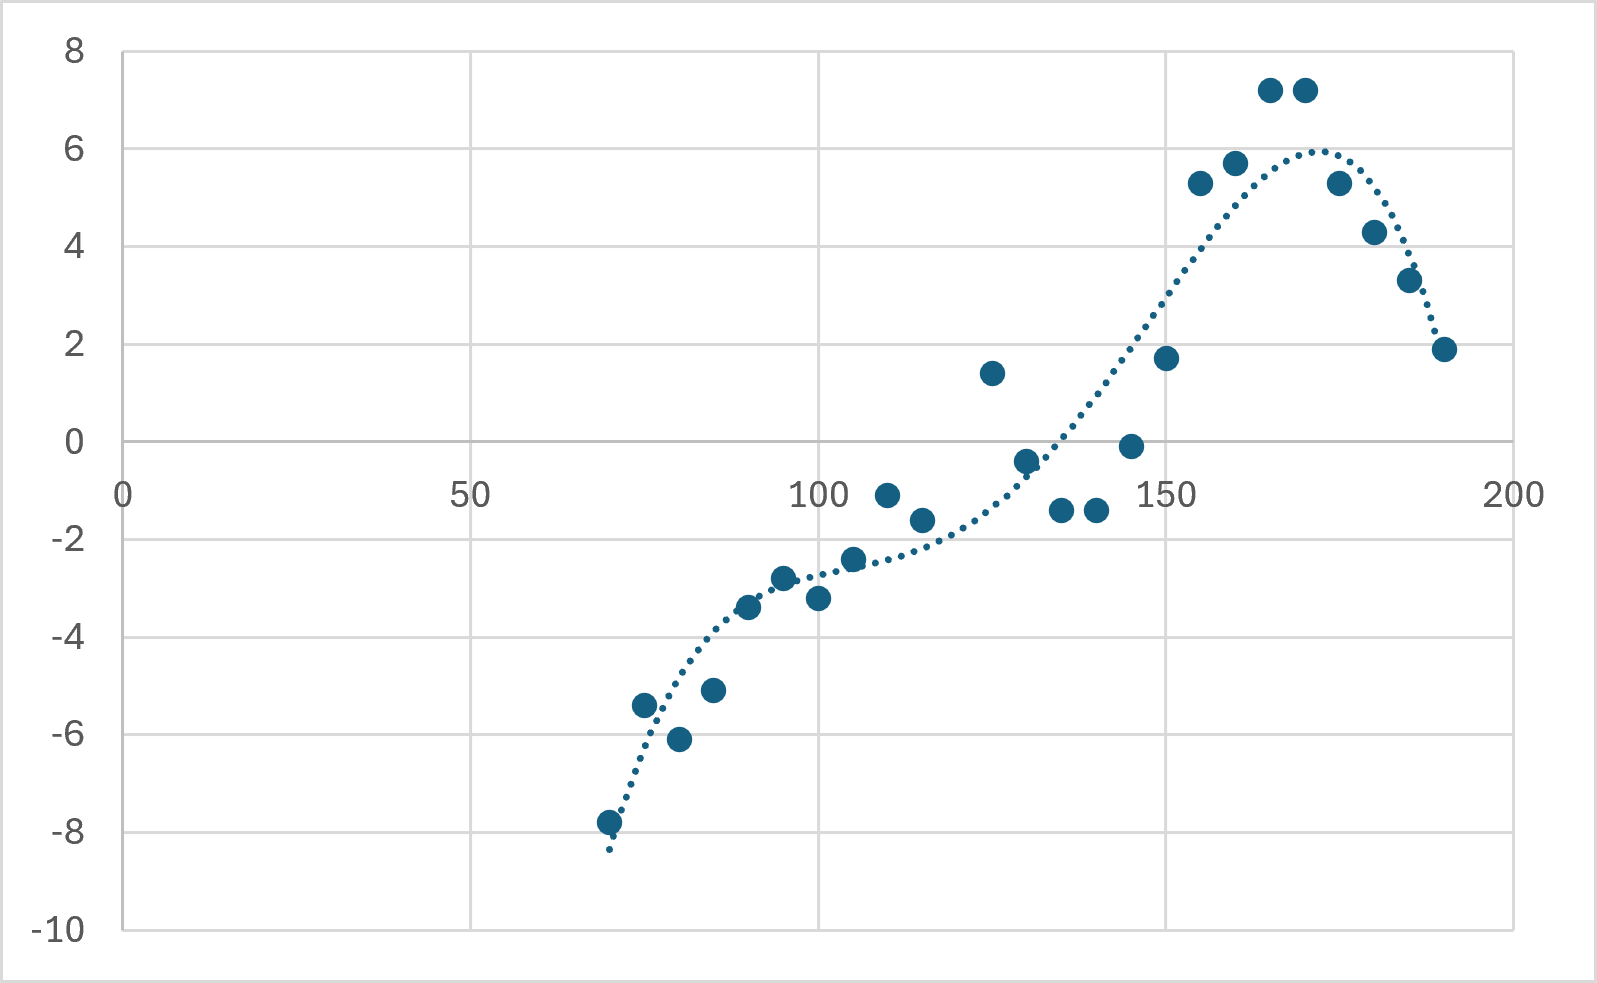
\includegraphics[width=\linewidth]{Polynomial.png}
   \caption{Diagram of the error based on real distance}
   \label{fig:Polynomial}
\end{figure}

Using the Excel trendline tool, we got this error equation:

\begin{equation}
\begin{split}
   f(x) ={}& -1.004 \times 10^{-6}\, x^4 + 0.0005059\, x^3 \\
           & - 0.09263\, x^2 + 7.398\, x - 221.7
\end{split}
\end{equation}

Every measure passes through the equation and is recalibrated based on it.
That allows us to reduce the error when we are more than $\pm$10~cm from the
reference.



\subsubsection{Non Light Of Sight (NLOS) Filter}
Electromagnetic signals are very sensitive to obstacles. After doing research,
we have discovered that the signal loses power if it encounters an obstacle.
Based on that, we can verify that the power of the received signal is strong
enough; otherwise, the value cannot be considered as valid and we can reject it.

\subsubsection{Innovation gate filter}
UWB has a tendency to be noisy, which can create absurd values, either very
high or very low. These data can affect the controller and create some
discontinuities in the drone control. Based on the maximum speed of the drone,
we can determine absurdity by calculating the difference between the previous
distance $d_{-1}$ and the current $d$, then determining whether this difference
can be reached at the maximum speed. If not, the measure is ignored; otherwise,
we accept it.

\section{Communication Protocol} \label{COM_Protocol}

Drone to maintain formation requires various information, from its own sensors but also from the others drones. Drone also needs to transmit its data to a base and receive commands from it. To respond to this requirement, we implemented  ESP-NOW, a wireless communication protocol. 


\subsection{Formation Control}

The previous parts established a robust manner of collecting distance measurements through UWB as well as an efficient communication protocol for ESP boards with ESP-NOW. Along with the data from the flight controller's onboard sensors, the swarm can now collectively take advantage of many different information for its navigation. The objective is now to design a formation controller so that the swarm keeps a defined formation along a given trajectory.

\subsection{Formation Control}

The leader-follower architecture has been chosen for its ease of implementation and to limit the transmission of data. The idea is the following : the leader is given a trajectory to follow, for example navigating between two waypoints, and the two followers adjust themselves to follow the leader while keeping the formation. This implies that the leader doesn't take part in the formation control as its only goal is to reach its destination : that reduces the overall complexity of the system.


The chosen formation control architecture relies on a distance-based control which basically has the goal of keeping a specified distance between each drone at any given moment. The chosen control law is based on a PD controller (Proportional-Derivative) and can be explained with a simple analogy using a spring : the proportional term corresponds to the restoring force of the spring while the derivative term is comparable to the damping factor of the spring.

Let's consider a triangle formation made of 3 drones. Each edge of the triangle is modelled by a spring whose resting length is equivalent to the desired distance $d_{des}$ between the 2 drones. The 2 neighbours $j\in[1,2,3]$ of each drone $i\in[1,2,3]$ belong to $\mathcal{N}_i$.

\begin{itemize}
    \item The restoring force pushes or pulls the drone to minimize the distance error :

    \begin{equation}
       P=-K_p\sum_{j\in \mathcal{N}_i}(d_{ij}-d^\ast _{ij})\frac{p_i-p_j}{d_{ij}}
    \end{equation}
    

    $K_p$ is the proportional gain, $d_{ij}$ is the distance between drone $i$ and drone $j$, $d^\ast_{ij}$ is the \textbf{desired} distance between drone $i$ and drone $j$, $p_i-p_j$ is relative position vector. Dividing it by the distance between the drones gives us a normalized vector pointing in the direction between the 2 drones. We sum the force obtained for each neighbour of the drone to get the overall vectorial force. The proportional term therefore generates a force in the right direction depending on the distance error : if $d_{ij}>d^\ast _{ij}$ then the drone is too far and the overall force is negative. Since the relative position vector is pointing from drone  $j$ to drone $i$, the negative force pushes drone $i$ towards drone $j$. If $d_{ij}<d^\ast _{ij}$, the overall force is positive and pulls drone $i$ away from drone $j$.

    
    \item The damping force allows to minimize the oscillations and avoid collisions :
    \begin{equation}
        D=-K_d\sum_{j\in \mathcal{N}_i}(v_i-v_j)
    \end{equation}
    

    $K_p$ is the derivative gain, $v_{i}$ and $v_j$ are respectively the velocities of drone $i$ and drone $j$. If the difference between the velocities of the drones is too large, the derivative term generates an opposite force to slow the movement. We do the sum of the force for each neighbouring drone to get an overall force.

    \item The final total control input $u$ for drone $i$ is : 
    \begin{equation}
          u_i=-K_p\sum_{j\in \mathcal{N}_i}(d_{ij}-d^\ast _{ij})\frac{p_i-p_j}{d_{ij}}-K_d\sum_{j\in \mathcal{N}_i}(v_i-v_j)
    \end{equation}
  
\end{itemize}

This control law implies that each follower drone  should be able to make the following measurements :

\begin{itemize}
    \item $d$ : the distances between itself and the other drones (2 measurements per drone in a 3-drone swarm)
    \item $p$ : the relative position vector between itself and other drones
    \item $v$ : its own velocity and the velocity of its neighbours    
\end{itemize}

The distances can be retrieved thanks to the UWB sensors placed on the drones. On the other side, the velocities are estimated through the onboard EKF of the flight controller and can be easily communicated to the drone's neighbours through ESP-NOW as explained previously. Finally, we need to get the relative position vector defined by $p_i-p_j$. That data is not available directly therefore it is necessary to implement a state observer.


\subsection{State observer}

As its name suggests, a state observer is a model helping to reconstruct a state to be used in a state-space closed-loop model. This can be done in several manners and the Kalman Filter is one of the main possibilities. In this project, we propose to implement a simple Prediction-Correction algorithm (close to a Kalman Filter) to estimate the relative position vector. It is built as follows :

\begin{itemize}
    \item The prediction phase used a simple kinematic model to predict the relative position vector :
    $$\hat{p}_{pred}=\hat{p}+v_{rel}\cdot dt$$

    Here $\hat{p}_{pred}$ is the predicted vector, $\hat{p}$ is the previous step's estimation, $v_{rel}$ is the relative speed between 2 drones and $dt$ is the time step.

    \item The correction phase introduces the UWB measurement of the distance between the 2 drones $d_{mes}$ as follows : 
    \begin{equation*}
        \hat{p}= \hat{p}_{pred}+\frac{\hat{p}_{pred}}{\Vert \hat{p}_{pred}\Vert} \cdot l_{obs} \cdot (d_{mes}-\Vert \hat{p}_{pred}\Vert)
    \end{equation*}

    The observer gain $l_{obs}$ dictates how much we trust the UWB measurements to adjust the prediction. As these measurements are purely distances, we need to give it a direction which is made by multiplying by the fraction of the predicted vector by its norm. 

    \subsection{Full control and observer architecture}

\end{itemize}

\section{Visualization}
Drones are typically working far away from the operator. It makes it difficult
to observe and understand what is happening. That is a problem for testing
purposes, so we have to develop a visualizer which allows us to observe the
drones and detect errors and their causes. This visualizer uses MATLAB and is
based on ESP-NOW [\ref{COM_Protocol}].

We have developed an application which allows us to show different aspects.
Firstly, an attitude visualizer:
\begin{figure}[H]
   \centering
   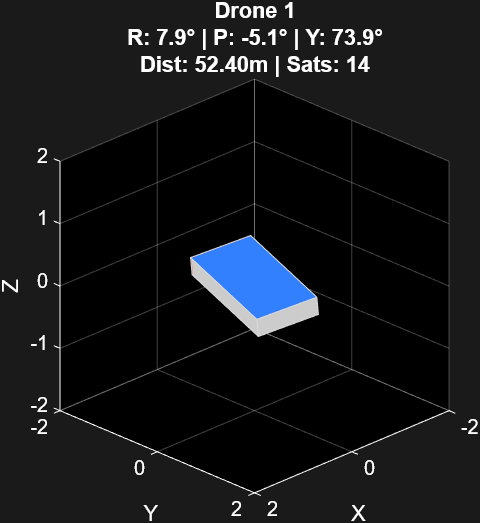
\includegraphics[width=\linewidth, height=5cm, keepaspectratio]{Attitude_visualization.png}
   \caption{Attitude visualizer}
   \label{fig:Attitude}
\end{figure}

Secondly, a formation visualizer:
\begin{figure}[H]
    \centering
    \begin{minipage}{0.48\linewidth}
        \centering
        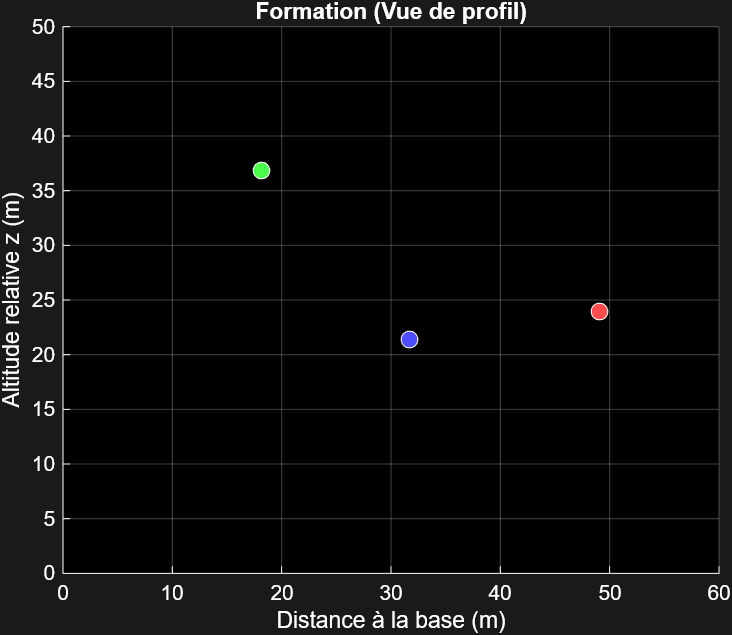
\includegraphics[width=\linewidth]{Formation_profil.png}
        \subcaption{Formation profile visualizer}
        \label{fig:FormationProfile}
    \end{minipage}\hfill
    \begin{minipage}{0.48\linewidth}
        \centering
        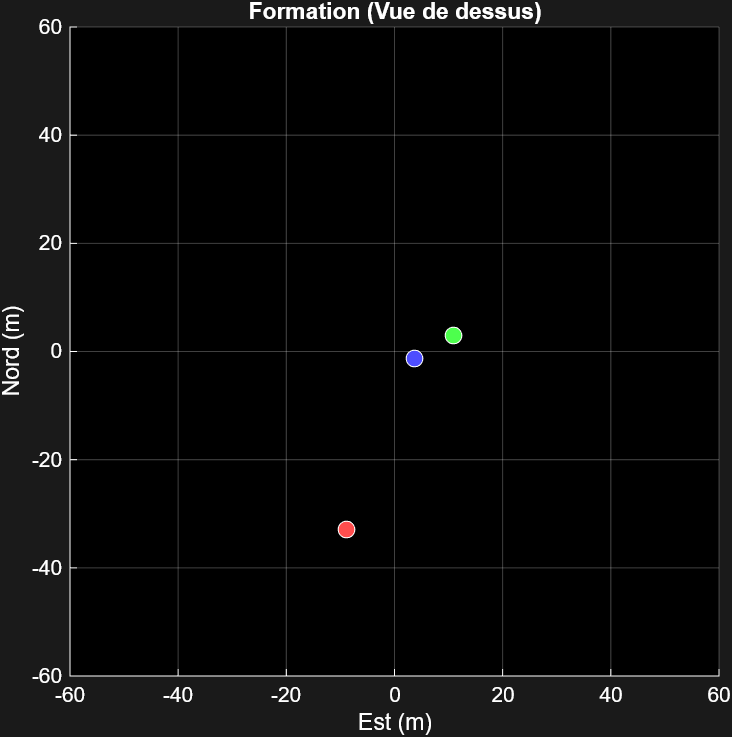
\includegraphics[width=\linewidth]{Formation_up.png}
        \subcaption{Formation upper view visualizer}
        \label{fig:FormationUp}
    \end{minipage}
    \caption{Formation visualizers}
    \label{fig:Formation}
\end{figure}

Then, a data visualizer:
\begin{figure}[H]
   \centering
   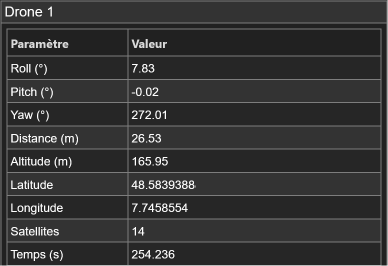
\includegraphics[width=\linewidth]{data_visualizer.png}
   \caption{Data visualizer}
   \label{fig:DataVisualizer}
\end{figure}




\section{Simulation}
Drones are restricted from flying above city. Moreover, our school does not have indoor test room. Those constraints reduce the number of outdoor test. However, test is necessary so we developed a simulation architecture. It is based on the flight controller firmware, Ardupilot, a proxy, MAVproxy and a visualizer, Mission planner.

\section{Conclusion}

\section*{References}

\end{document}
